\section{Outline}
This chapter investigates the effect of network structure on observed cooperation for the linear PGG described in \ref{ToTC}. The first section uses a simple lottery game to demonstrate the implementation of replicator dynamics. To this end, the paper \cite{RN30} is replicated and extended. \\

Then replicator dynamics are applied to the linear PGG. Under this regime, it is found that graphs with a power-law degree size distribution exhibit higher cooperation, when controlling for mean degree $m$. It is hypothesised that nodes with low degree size cooperate more, and the family of power-law models are characterised by a large number of low-degree nodes, resulting in higher overall cooperation than the WS and RRG model. \\
\section{Proof of Concept: Replicator and Imitation Dynamics} \label{Lottery_Me}
\subsection{Outline}
The paper chosen to replicate imitation and replicator dynamics was \cite{RN30}, which models a two-stage lottery game. Refer to \ref{Lottery} for a description of the game and the strategy space $S$. \\

The paper implemented agent-based replicator $(\alpha = 1)$ and imitation $(\alpha = 0)$ dynamics. After each round, every agent $i$ randomly chooses another agent $j$ from the population, and calculates $q_{i\to j}$, \\

\begin{equation} \label{rep}
q_{i\to j} = \Bigg[ \frac{|\pi_j - \pi_i|}{\Delta} \Bigg]^\alpha \mathbbm{1}_{\{\pi_j>\pi_i\}}, \quad  0 \leq \alpha \leq 1.\end{equation} 

In this formulation, $\Delta$ scales the difference so that $0 \leq q_{i\to j} \leq 1$, and $\Delta = 16$ in this two-stage lottery game. Each agent then changes from strategy $i$ to strategy $j$ if $q_{i\to j} \geq R,$ $R  \sim \mathsf{U}(0,1)$. A strategy $i$ has an \emph{evolutionary advantage} over strategy $j$, denoted $j \prec i$, if $q_{j \to i} >q_{i \to j}$.    \\

\subsection{Results Comparison}
The simulated results were compared to the paper for $\alpha = 0, 1$, and $ 0.5$, and are shown below. Each model consists of $N=6000$ agents, and each parameter permutation is simulated $T=100$ times. \\

\FloatBarrier 
\begin{figure}[!h]
  \begin{subfigure}[b]{0.45\textwidth}
    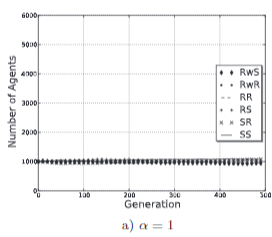
\includegraphics[width=\textwidth]{images/lottery1.png}
    \caption{Figure 5a from \cite{RN30}. The strategies SS, RR, SR, RS, R--WR, R--WS are represented by a solid line, crosses, plusses, dashes, dots and diamonds respectively. }
    \label{lottery1}
  \end{subfigure}
  \hfill
  \begin{subfigure}[b]{0.45\textwidth}
    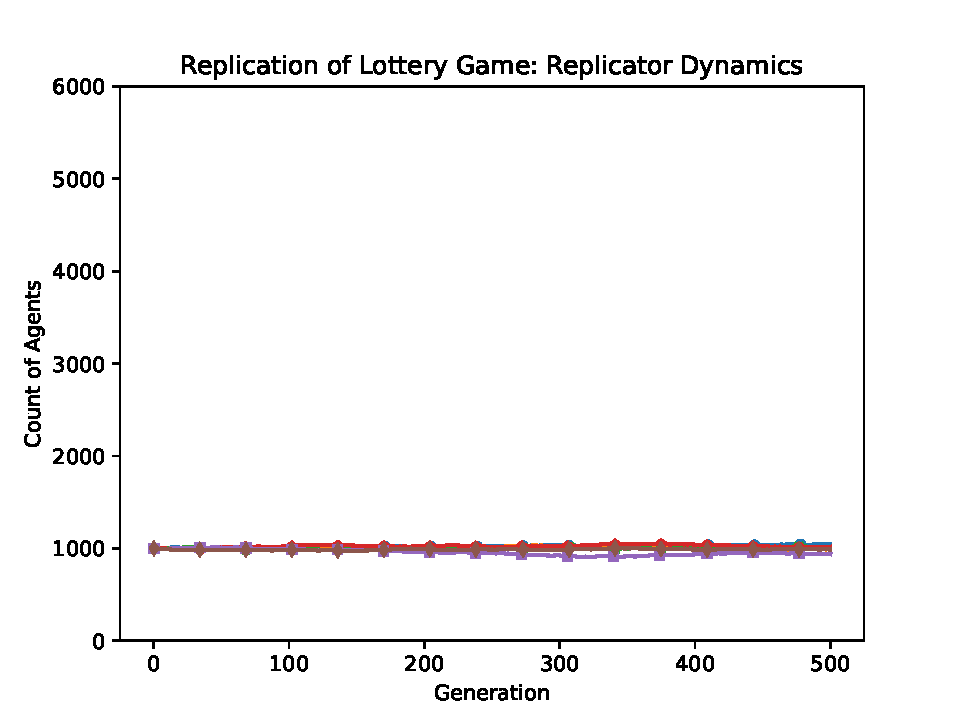
\includegraphics[width=1.25\textwidth]{images/lottery1_me.pdf}
    \caption{Replication of \ref{lottery1}. The strategies SS, RR, SR, RS, R--WR, R--WS are represented by blue circles, orange stars, green crosses, red pentagons, brown diamonds, and purple squares respectively.}
    \label{lottery1_me}
  \end{subfigure}
  \caption{Replication of Figure 5a from \cite{RN30}. The replication is successful, but these conditions do not provide anything interesting regarding replicator dynamics.  } \label{lottery_comp0}
\end{figure} 
\FloatBarrier
Under replicator dynamics, strategy $i$ has an evolutionary advantage over strategy $j$ if $\mathbb E [\pi_i] >\mathbb E [\pi_j]$. Because the expected value of the strategies considered in Figure \ref{lottery_comp0} are equal, no strategy has an evolutionary advantage over any other, so the initial distribution of strategies remains.
\FloatBarrier 
\begin{figure}[!h]
  \begin{subfigure}[b]{0.45\textwidth}
    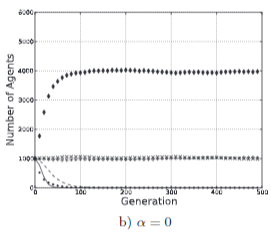
\includegraphics[width=\textwidth]{images/lottery2.png}
    \caption{Figure 5b from \cite{RN30}. The strategies SS, RR, SR, RS, R--WR, R--WS are represented by a solid line, crosses, plusses, dashes, dots and diamonds respectively. }
    \label{lottery2}
  \end{subfigure}
  \hfill
  \begin{subfigure}[b]{0.45\textwidth}
    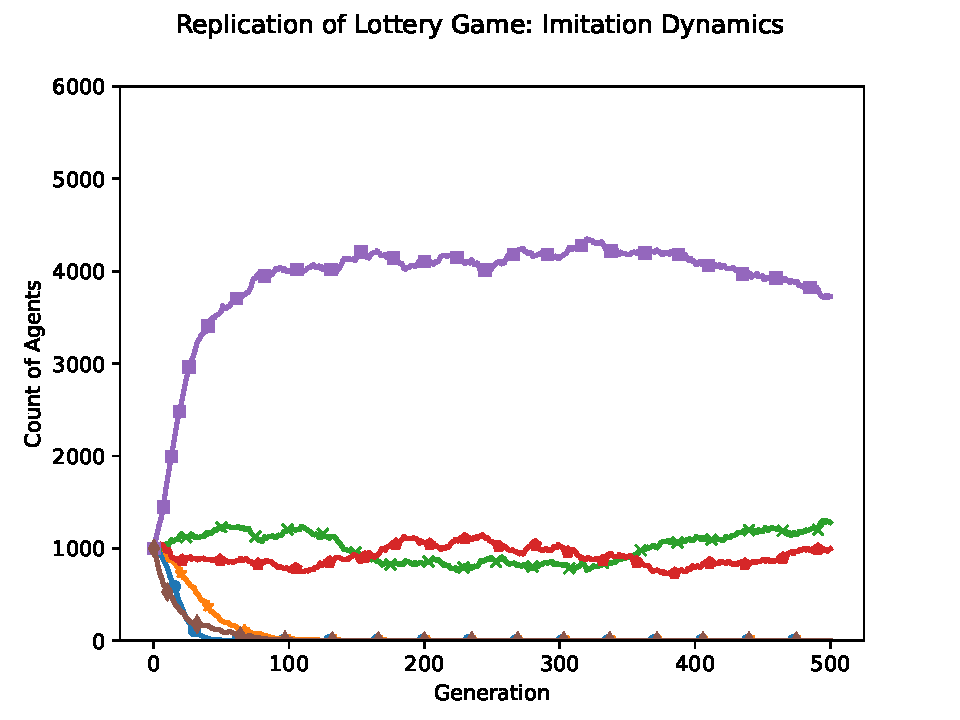
\includegraphics[width=1.25\textwidth]{images/lottery2_me.pdf}
    \caption{Replication of \ref{lottery2}. The strategies SS, RR, SR, RS, R--WR, R--WS are represented by blue circles, orange stars, green crosses, red pentagons, brown diamonds, and purple squares respectively.}
    \label{lottery2_me}
  \end{subfigure}
  \caption{Replication of Figure 5b from \cite{RN30}. Strategies RS and SR have no evolutionary advantages or disadvantages relative to other strategies, so they persist. However R--WS $\prec$ SS, RR, and R--WR, and they are sent extinct.} \label{lottery_comp1}
\end{figure} 
\FloatBarrier



\FloatBarrier 
\begin{figure}[!h]
  \begin{subfigure}[b]{0.45\textwidth}
    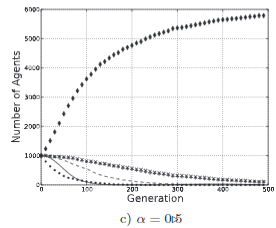
\includegraphics[width=\textwidth]{images/lottery3.png}
    \caption{Figure 5c from \cite{RN30}. The strategies SS, RR, SR, RS, R--WR, R--WS are represented by a solid line, crosses, plusses, dashes, dots and diamonds respectively. }
    \label{lottery3}
  \end{subfigure}
  \hfill
  \begin{subfigure}[b]{0.45\textwidth}
    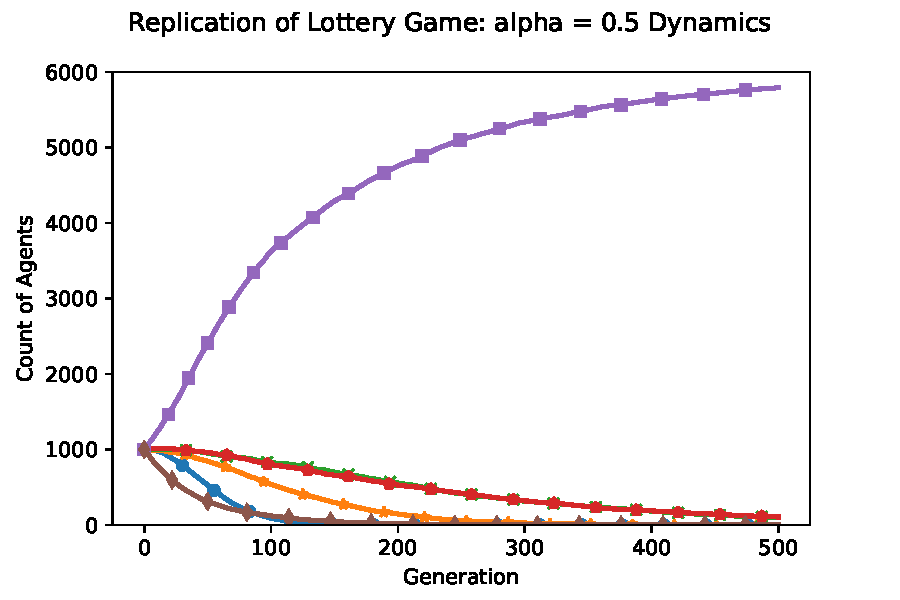
\includegraphics[width=1.25\textwidth]{images/lottery3_me.pdf}
    \caption{Replication of \ref{lottery3}. The strategies SS, RR, SR, RS, R--WR, R--WS are represented by blue circles, orange stars, green crosses, red pentagons, brown diamonds, and purple squares respectively. }
    \label{lottery3_me}
  \end{subfigure}
  \caption{Replication of Figure 5c from \cite{RN30}. This is neither true imitation or replicator dynamic, but provides an intermediary case. The replicated results emulate the paper \cite{RN30}, so the replication is successful. In the $\alpha = 0.5$ regime, R--WS has an evolutionary advantage over all other strategies, and sends them all to extinction. The time to extinction for each strategy depends on the magnitudes of the evolutionary advantages. } \label{lottery_comp2}
\end{figure} 
\FloatBarrier
The results are well replicated for all $\alpha$, and this model for evolutionary dynamics can be explored on other games. To transpose this model onto a network, it is necessary to restrict the sample space of each agent to its network neighbours. \\

 It is also interesting to examine the results when the lottery win probability $p$ is not 0.5. For replicator dynamics, the strategy with the highest expected value eventually wins out, because it will have an evolutionary advantage. For imitation dynamics the result is not so obvious. This was shown in Figure 6 from \cite{RN30}, and replicated below. For $p=0.4$, the expectation-maximising strategy is SS, but R--WS has an evolutionary advantage and takes over the population. This is supported by theoretical results in \cite{RN30}.  \\
 
 \FloatBarrier 
\begin{figure}[!h]
  \begin{subfigure}[b]{0.45\textwidth}
    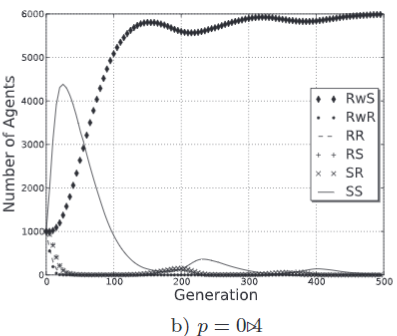
\includegraphics[width=\textwidth]{images/lotteryp4.png}
    \caption{Figure 6b from \cite{RN30}. The strategies SS, RR, SR, RS, R--WR, R--WS are represented by a solid line, crosses, plusses, dashes, dots and diamonds respectively.}
    \label{lotteryp4}
  \end{subfigure}
  \hfill
  \begin{subfigure}[b]{0.45\textwidth}
    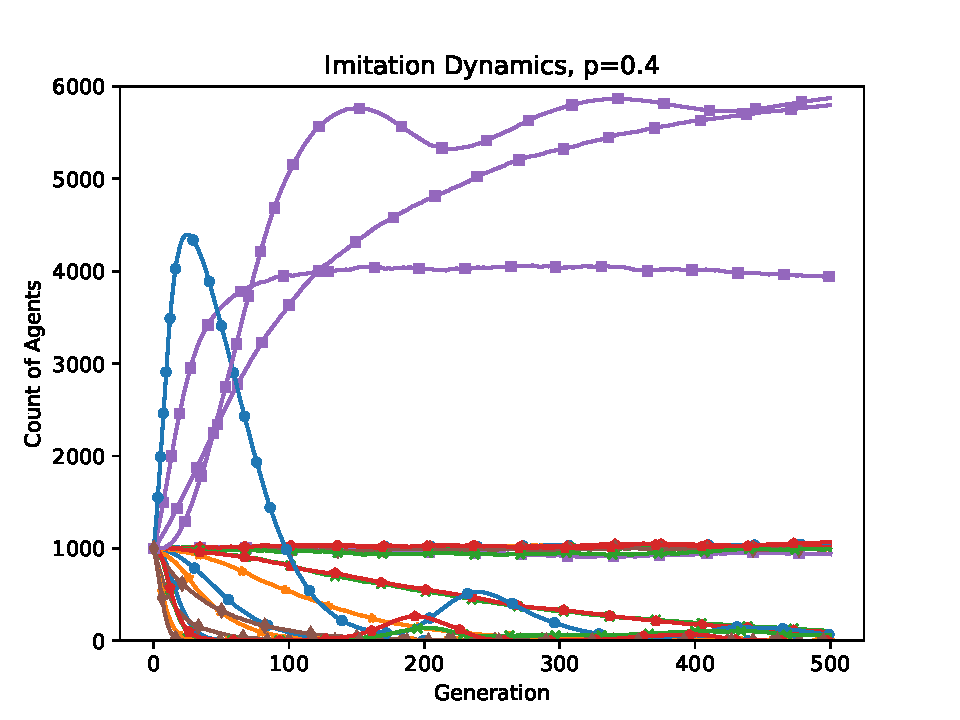
\includegraphics[width=1.25\textwidth]{images/lotteryp4_me.pdf}
    \caption{Replication of \ref{lotteryp4}. The strategies SS, RR, SR, RS, R--WR, R--WS are represented by blue circles, orange stars, green crosses, red pentagons, brown diamonds, and purple squares respectively. }
    \label{lotteryp4_me}
  \end{subfigure}
  \caption{Replication of Figure 6b from \cite{RN30}. Although SS is the expectation--maximising strategy, it is not an ESS, and R--WS eventually dominates the population. The parameter $p$ dictates the probability of winning a round of the lottery. For $p=0.4$, $\mathbb E [\pi_{\text{SS}}] = 8$, and $\mathbb E [\pi_{\text{R--WS}}] =6.72 $.} \label{lottery_comp4}
\end{figure} 
\FloatBarrier
Similarly, for $p=0.55$, the expectation--maximising strategy is RR, but R--WS also takes over the population.\\
 \FloatBarrier 
\begin{figure}[!h]
  \begin{subfigure}[b]{0.45\textwidth}
    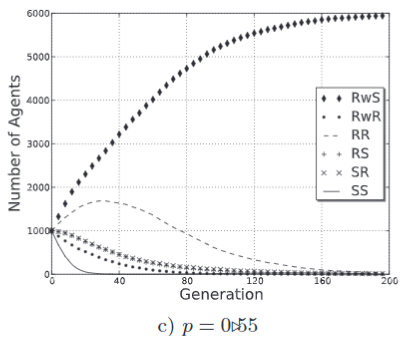
\includegraphics[width=\textwidth]{images/lotteryp055.png}
    \caption{Figure 6c from \cite{RN30}. The strategies SS, RR, SR, RS, R--WR, R--WS are represented by a solid line, crosses, plusses, dashes, dots and diamonds respectively.}
    \label{lotteryp055}
  \end{subfigure}
  \hfill
  \begin{subfigure}[b]{0.45\textwidth}
    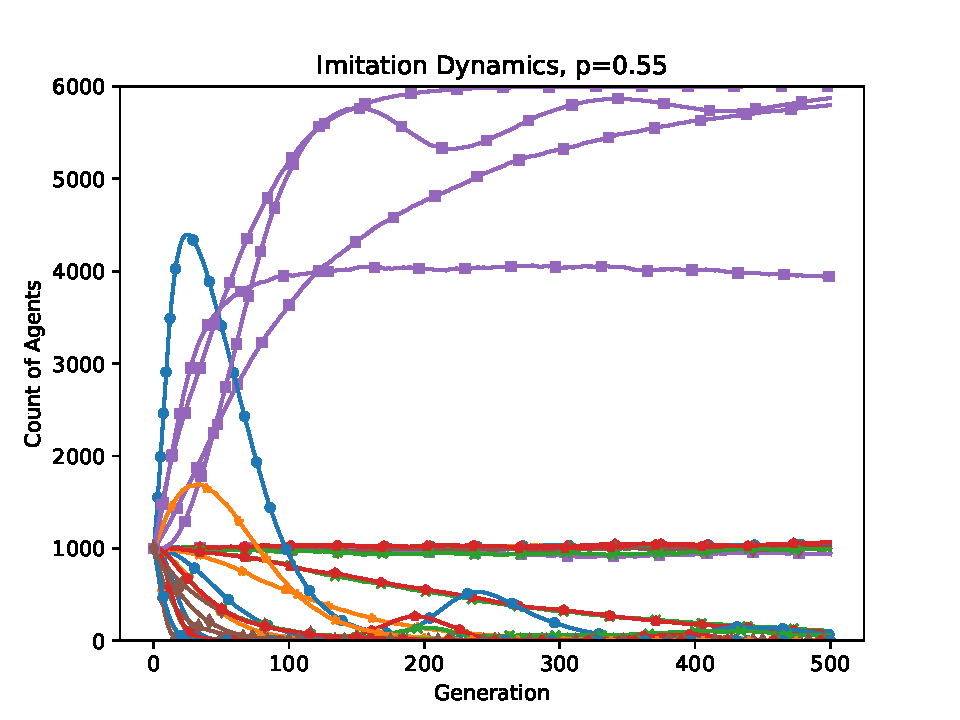
\includegraphics[width=1.25\textwidth]{images/lotteryp055_me.pdf}
    \caption{Replication of \ref{lotteryp055}. The strategies SS, RR, SR, RS, R--WR, R--WS are represented by blue circles, orange stars, green crosses, red pentagons, brown diamonds, and purple squares respectively. }
    \label{lotteryp4_me_2}
  \end{subfigure}
  \caption{Replication of Figure 6c from \cite{RN30}. In this case, RR is expectation-maximising because $p>0.5$, but R--WS still takes over the population. The initial spike of RR is due to its evolutionary advantage over the strategies SS, SR, RS, and R--WR.  For $p=0.55$, $\mathbb E [\pi_{\text{RR}}] = 8.8$, and $\mathbb E [\pi_{\text{R--WS}}] =8.58 $.} \label{lottery_comp5}
\end{figure} 
\FloatBarrier
In \cite{RN30}, plots for $p=0.3, 0.7$ were also shown, however the expectation--maximising strategies win out quickly, so they are not included here. It is notable that in Figure \ref{lotteryp4_me}, there are some fluctuations that occur before stability. This is investigated further. \\
\subsection{Extension: Deterministic Model}


Under the $p=0.4$ regime, the probability distribution for each strategy is calculated. \\
 \begin{align*}
 \mathbb P_{\text{SS}}(x = \pi)  &= \mathbbm{1}_{\pi = 8}, \\
 \mathbb P_{\text{RR}}(x = \pi)  &= \begin{cases} 0.36 \quad \pi = 0 \\
    0.48 \quad \pi =8 \\ 0.16 \quad \pi = 16
    \end{cases}, \\
    \mathbb P_{\text{RS}}(x = \pi)  &= \begin{cases} 0.6 \quad \pi =4  \\
     0.4 \quad \pi = 12
    \end{cases}, \\
    \mathbb P_{\text{SR}}(x = \pi)  &= \begin{cases} 0.6 \quad \pi =4  \\
     0.4 \quad \pi = 12
    \end{cases}, \\
        \mathbb P_{\text{R--WS}}(x = \pi)  &= \begin{cases} 0.36 \quad \pi = 0 \\
    0.24 \quad \pi =8 \\
    0.4 \quad \pi = 12\\
    \end{cases}, \\
    \mathbb P_{\text{R--WR}}(x = \pi)  &= \begin{cases} 0.6 \quad \pi = 4 \\
    0.24 \quad \pi =8 \\
    0.16 \quad \pi = 16\\
    \end{cases}, \\
\end{align*}
Under imitation dynamics, a strategy $i$ has an evolutionary advantage over $j$, if $\mathbb P(\pi_i > \pi_j) > \mathbb P(\pi_i < \pi_j)$. In the $p=0.4$ case, RS $\prec$ SS $\prec$ R--WS $\prec$ RS, which is a cycle. However, the magnitude of the evolutionary advantage also has an effect. In Figure \ref{lotteryp4_me}, the strategy SS eliminates RS much faster than RS can eliminate R--WS, so SS temporarily grows, and then succumbs to R--WS. \\

This relationship can be expressed as a set of difference equations. Call $\rho_{i,t}$ the proportion of strategy $i$ present at time $t$. The boundary condition is $\sum_i \rho_{i,t}= 1$, $\forall t \in [0,T]$. Denote $\mathcal F_t$ the natural filtration of $\cap_i \{\rho_{i,t} \}$ at time $t$. \textbf{THIS NEEDS TO BE INTERSECTION OF NATURAL FILTRATIONS}  \\
\begin{align*}
    \mathbb E \big [\rho_{\text{SS},t+1}| \mathcal F_t \big ] &= \rho_{\text{SS},t} \Bigg [\sum_{ i \neq \text{SS}}  \rho_{\text{i},t} [\mathbb P (\pi_\text{SS} > \pi_{i}) -\mathbb P (\pi_\text{SS} < \pi_{i}) ] \Bigg ] \\
    &= \rho_{\text{SS},t}\Bigg [\rho_{\text{RR}, t}(0.36-0.16) + \rho_{\text{RS}, t}(0.6-0.4) + \rho_{\text{SR}, t}(0.6-0.4) + \\
     & \quad \rho_{\text{R--WS}, t}(0.36-0.4) + \rho_{\text{R--WR}, t}(0.6-0.16) \Bigg ] \\
    &= \rho_{\text{SS},t}\Bigg [\rho_{\text{RR}, t}(0.2) + \rho_{\text{RS}, t}(0.2) + \rho_{\text{SR}, t}(0.2) + 
      \quad \rho_{\text{R--WS}, t}(-0.04) + \rho_{\text{R--WR}, t}(0.44) \Bigg ] \\
\end{align*}
The same logic can be applied for each strategy, which results in a difference equation for each strategy, \\
\begin{align*}
    \mathbb E \big [\rho_{\text{RR},t+1}| \mathcal F_t \big ] &=\rho_{\text{RR},t}\Bigg [\rho_{\text{SS}, t}(-0.2) + \rho_{\text{RS}, t}(-0.104) +  \rho_{\text{SR}, t}(-0.104) + \\ & \rho_{\text{R--WS}, t}(-0.0896) + \rho_{\text{R--WR}, t}(-0.0144) \Bigg ], \\
    \mathbb E \big [\rho_{\text{RS},t+1}| \mathcal F_t \big ] &=\rho_{\text{RS},t}\Bigg [\rho_{\text{SS}, t}(-0.2) + \rho_{\text{RR}, t}(0.104) +  \rho_{\text{SR}, t}(0) + \\ & \rho_{\text{R--WS}, t}(0.072) + \rho_{\text{R--WR}, t}(0.032) \Bigg ] ,\\
    \mathbb E \big [\rho_{\text{SR},t+1}| \mathcal F_t \big ] &=\rho_{\text{SR},t}\Bigg [\rho_{\text{SS}, t}(-0.2) + \rho_{\text{RR}, t}(0.104) +  \rho_{\text{RS}, t}(0) + \\ & \rho_{\text{R--WS}, t}(0.072) + \rho_{\text{R--WR}, t}(0.032) \Bigg ] ,\\
    \mathbb E \big [\rho_{\text{R--WS},t+1}| \mathcal F_t \big ] &=\rho_{\text{R--WS},t}\Bigg [\rho_{\text{SS}, t}(0.04) + \rho_{\text{RR}, t}(0.0896) +  \rho_{\text{SR}, t}(-0.072) + \\ & \rho_{\text{RS}, t}(-0.072) + \rho_{\text{R--WR}, t}(0.032) \Bigg ] , \\
\mathbb E \big [\rho_{\text{R--WR},t+1}| \mathcal F_t \big ] &=\rho_{\text{R--WR},t}\Bigg [\rho_{\text{SS}, t}(-0.44) + \rho_{\text{RR}, t}(0.0144) +  \rho_{\text{SR}, t}(-0.032) + \\ & \rho_{\text{RS}, t}(-0.032) +\rho_{\text{R--WS}, t}(-0.032)  \Bigg ] , \\    
\end{align*}

This set of difference equations cannot be solved analytically, however the numerical simulation is investigated. \\
\FloatBarrier
\graphCap{ODE_lottery.pdf}{0.75}{Deterministic Simulation of the Lottery Game. The strategies SS, RR, SR, RS, R--WR, R--WS are represented by blue circles, orange stars, green crosses, red pentagons, brown diamonds, and purple squares respectively. The starting condition is $\rho_{i,0} = \tfrac{1}{6}$, for each strategy $i$. Initially, it reports similar results to the stochastic model, however the deterministic model is cyclical, and no strategies are eliminated. Note that SR and RS are identical, so the green series is covered by the red series. }{ODE_lottery}
\FloatBarrier
A major difference between the $p=0.4$ stochastic model and its deterministic extension is the ability for strategies to go extinct. In the stochastic model, extinction is possible, particularly when the proportion of that strategy is already close to 0. Furthermore, once a strategy is extinct it can never return. For example, at the trough of the RS strategy, it represents 0.04\% of the population. This corresponds 2.5 agents in the simulations. It is feasible that both these agents go extinct, and the RS strategy is eliminated. In the difference equations model, no strategy can ever go extinct. The elimination of RS ensures the eventual dominance of R--WS. RR is eliminated quickly because it has the highest pairwise death rate, as SS dominates it with a rate of 0.44. This is much larger than any other pairwise comparison rate.  \\


\subsection{Extension: Robustness} 
The effect of extinction also affects the robustness of results. Some trials may eliminate strategies at their first trough, whereas these strategies may survive much longer in other trials. Therefore the empirical quantiles are examined.\\
\FloatBarrier
\graphCap{lotteryp4_me_quantiles_empirical.pdf}{0.75}{Empirical 2.5\%, 97.5\% Quantiles of Imitation Dynamics Lottery Game, $p=0.4$, $T = 100$. The strategies SS, RR, SR, RS, R--WR, R--WS are represented by blue circles, orange stars, green crosses, red pentagons, brown diamonds, and purple squares respectively. The quantile for each series is the dashed line. }{lottery_quantiles_empirical}
\FloatBarrier
Figure \ref{lottery_quantiles_empirical} shows how great the variance of certain series are, particularly SS and R--WS. When R--WS is prominent and the strategies SR, RS are not extinct, SR and RS are able to grow. This occurs around the 200th generation. The strategy SS, which outperforms SR and RS, then dominates them. SS is dominated by R--WS, and this cycle continues until SR and RS are eliminated. The reason that they are eliminated is because the highest rate of dominance is SS over SR, RS. The empirical quantile plots exhibit a second trough, similar to Figure \ref{ODE_lottery}, however only the beginning of a third trough is shown.  \\
\FloatBarrier
\graphCap{lotteryp4_me_quantiles.pdf}{0.75}{95\% Confidence Interval for the Mean, Imitation Dynamics Lottery Game, $p=0.4$, $T = 100$. The strategies SS, RR, SR, RS, R--WR, R--WS are represented by blue circles, orange stars, green crosses, red pentagons, brown diamonds, and purple squares respectively. The confidence interval for each series is the dashed line. }{lottery_quantiles}
\FloatBarrier
 The computed confidence intervals assume a normal distribution of the mean under the Central Limit Theorem. The computed standard deviation of each point in the time series is used as an estimate of the true standard deviation. Because the number of trials $T=100$, the confidence interval is tight around the sample mean. The original paper uses $T=20$, which results in a confidence interval more than four times as wide Figure \ref{lottery_quantiles}. Therefore it is suggested that more than 20 trials are used for future samples. \\



\subsection{Summary}
The purpose of replicating \cite{RN30} was to demonstrate replicator and imitation dynamics. This demonstration was achieved, and now these dynamics can be applied to the PGG. A cycle of strategies was demonstrated for imitation dynamics under a $p=0.4$ regime. Although the original paper did not investigate the distribution of results, they are discussed above. The paper \cite{RN30} did not use an underlying network structure, but the dynamics can easily be transposed onto a graph by limiting the sample space of agents to neighbours. \\


\section{Local Replicator Dynamics for Public Good Games}
\subsection{Outline}
The following section investigates the effect of the graph model on cooperation under local replicator dynamics. The graph models from \ref{other_networks} are also investigated here, and sample characteristics are given in Table \ref{graph_stats}. The game is played by a population of 500 agents, where each agents hosts a play of the PGG with their neighbours. After every agent has hosted, the agent-based replicator dynamics from equation \eqref{rep} are implemented for each agent. Each plot aggregates the mean of each series over 100 trials. \\

It is found that the graphs with a power-law degree size distribution induce higher cooperation. The effect of $C_\Delta$ is not initially evident when comparing the WS, BA, TAG, and RRG models, so a new model type, the power-law (PL) model, is introduced to examine the effect of $C_\Delta$ for scale-free degree size distributions. The effect of $C_\Delta$ is also examined in the WS family of graph models. Under the PL model, higher $C_\Delta$ weakly induces higher cooperation, while the trend is reversed for the WS family of models. \\

Then the effect of targeted mean degree $m$ is examined for RRG and BA models. Both of these experiments indicate that higher $m$ lead to lower cooperation. Finally, the cooperation levels are stratified by degree size within a BA graph model. \textbf{NO TREND YET} These experiments show that the nodes with low degree size have a higher contribution proportion than average, which may explain the trend. \\

\subsection{Results}
These results examine the effect of network model on cooperation. For consistency, the WS model has parameter $p=0.1$ and the TAG model has parameter $\alpha = 0.3$, which aligns with Chapter \ref{TA}. Replicator dynamics result in slower convergence than the satisfaction model in Chapter \ref{TA}. Therefore the number of generations has been extended to 200, so that equilibrium is observed. Figure \ref{replicator_low} shows the TAG and BA model inducing higher cooperation than WS, RRG models. This trend continues for $2.5 \leq r \leq 7.5$. It appears that graph models with a power law degree size distribution induce higher cooperation. \\
\FloatBarrier
\graphCap{replicator_new_low.pdf}{0.7}{Comparing Graph Models: Replicator Dynamics. Trend for $r \in \{4.0, 4.25, 4.5, 4.75\}$. In each graph, the blue circles, orange stars, green crosses, and red pentagons correspond to the WS model, TAG model, BA model, and RRG model respectively. It appears that the BA model induces the highest cooperation, then the TAG, followed by WS and RRG respectively. This corresponds to decreasing degree size variance. \textbf{WHY IS 4.75 BA SO HIGH} }{replicator_low} 
\FloatBarrier
\graphCap{replicator_new_med.pdf}{0.7}{Comparing Graph Models: Replicator Dynamics. Trend for $r \in \{5.0, 5.25, 5.5, 5.75\}$. In each graph, the blue circles, orange stars, green crosses, and red pentagons correspond to the WS model, TAG model, BA model, and RRG model respectively. For $r\geq 5.5$, the RRG model induces more cooperation than the WS model. }{replicator_medium}
\FloatBarrier
\graphCap{replicator_new_high.pdf}{0.7}{Comparing Graph Models: Replicator Dynamics. Trend for $r \in \{6,6.5,7,7.5\}$. In each graph, the blue circles, orange stars, green crosses, and red pentagons correspond to the WS model, TAG model, BA model, and RRG model respectively. The TAG and RRG models overtake the BA model, while the WS model consistently induces the lowest cooperation amongst models. }{replicator_large}\FloatBarrier



There is insufficient information to determine if the clustering coefficient $C_\Delta$ influences cooperation, because the graph models are too varied. Therefore, it will need to be tested in isolation.\\

\subsection{Isolating the Effect of Clustering Coefficient: Power Law Degree Size Distribution}
To test the hypothesis that the average clustering coefficient $C_\Delta$ does not impact cooperation, the \verb+power_law+ model was used to create another graph model, denoted PL. It induces a degree distribution with power law shape, but the parameter $p$ dictates the clustering coefficient. After each node is connected, the parameter $p$ determines the probability that the next link joins two neighbours, completing the triangle. Two degree histograms are plotted below, which emphasise the degree size distribution. \\
\FloatBarrier
\graphCap{PL01BA.pdf}{0.7}{Comparison of Power Law Clustering Graph with BA model, $p=0.1$. The degree histograms are similar, so the only difference is the clustering coefficient.}{PL01BA}
\FloatBarrier
\graphCap{PL05BA.pdf}{0.7}{Comparison of Power Law Clustering Graph with BA model, $p=0.5$. The degree histograms are similar, so the only difference is the clustering  coefficient.}{PL05BA}
\FloatBarrier
The summary statistics are also reported, with parameter $N = 500$ and targeted mean degree $m=6$. Both $C_\Delta$ and degree variance increase with respect to $p$. From \ref{graph_stats}, the BA model reports $l=3.24, C_\Delta = 0.05$, and a degree variance of 40.80. The major difference between a BA and PL model is $C_\Delta$, but the degree variance is also different and must be regarded.   \\
\FloatBarrier
\begin{table}[!h]
\begin{center}
\begin{tabular}{|l|l|l|l|l|}
\hline
Graph Type & Mean Degree & $l$ & $C_\Delta$ & Degree Variance \\ \hline
PL: $p=0.1$        & 5.96        & 3.234                         & 0.10                   & 42.35           \\ \hline
PL: $p=0.2$        & 5.96           & 3.24                         & 0.15                   & 44.07               \\ \hline
PL: $p=0.3$       & 5.96        & 3.23                       & 0.20                   & 46.28           \\ \hline
PL: $p=0.4$       & 5.96        & 3.25                         & 0.25                   & 47.92           \\ \hline
PL: $p=0.5$         & 5.96           & 3.26                         & 0.30                   & 50.47            \\ \hline
\end{tabular}
\caption{Computed characteristics for PL graph, varying cluster parameter $p$. The characteristics were computed over 100 samples of each graph, and then averaged. In each case, the targeted mean degree $m$ was set to 6. } \label{graph_stats_PL}
\end{center}
\end{table}
The PL model was tested, under a replicator dynamics regime, for a range of $r$. 
\FloatBarrier
\graphCap{comparing_power_p_low.pdf}{0.7}{To test the effect of $C_\Delta$, the parameter $p$ in a PL graph was varied. In each graph, the blue circles, orange stars, green crosses, red pentagons, and purple squares correspond to $p\in\{0.1,0.2,0.3,0.4,0.5\}$ respectively. The observed trend is that higher $p$, and hence higher $C_\Delta$ leads to marginally higher cooperation.}{power_p_low}
\FloatBarrier
\graphCap{comparing_power_p_high.pdf}{0.7}{To test the effect of $C_\Delta$, the parameter $p$ in a PL graph was varied. In each graph, the blue circles, orange stars, green crosses, red pentagons, and purple squares correspond to $p \in \{0.1,0.2,0.3,0.4,0.5\}$ respectively. The trend is unclear here, because $r=2.75, 3.5$ indicate higher $p$, and hence higher $C_\Delta$ leads to higher cooperation, but that trend is not observed for $r=3.0,3.25$.}{power_p_high} \FloatBarrier

These tests indicate that, when controlling for degree size distribution, the clustering coefficient $C_\Delta$ may have a marginal effect. The correlation is weakly positive, and is much more evident for $1.75\leq r\leq 3.0$. It is also necessary to test the effect of $C_\Delta$ under a different degree size distribution. \\

\subsection{Isolating the Effect of Clustering Coefficient: Constant Degree Size Distribution}
The WS model is a family of graphs characterised by rewiring probability $p$. By increasing $p$, the $l$ statistic is reduced while $C_\Delta$ remains high for $0\leq p\leq0.15$. However there exists a region for $p$ where $C_\Delta$ decreases and $l$ does not change as rapidly. It is this region that will be isolated to test the effect of local clustering on cooperation in graphs under a near-constant degree distribution regime. Recall that a WS graph starts with a circle of nodes, each node connected to its adjacent $\frac{m}{2}$ circular neighbours. Hence the initial degree is $m$ for each node, and this only varies marginally due to $p$. There are certainly no scale factors such as in the PL, BA, or TAG models. \\

\FloatBarrier
\begin{table}[!h]
\begin{center}
\begin{tabular}{|l|l|l|l|l|}
\hline
Graph Type & Mean Degree & $l$ & $C_\Delta$ & Degree Variance \\ \hline
WS: $p=0.1$        & 6        & 5.41                         & 0.44                  & 0.57           \\ \hline
WS: $p=0.2$        &6           & 4.53                         & 0.316                   & 1.06               \\ \hline
WS: $p=0.3$        &6           & 4.16                         & 0.22                   & 1.51               \\ \hline
WS: $p=0.4$       & 6        & 3.95                         & 0.14                  & 1.93           \\ \hline
WS: $p=0.5$         & 6           & 3.83                         & 0.09                   & 2.25            \\ \hline
\end{tabular}
\caption{Computed characteristics for WS graph, varying rewiring probability parameter $p$. The characteristics were computed over 100 samples of each graph, and then averaged. The targeted mean degree $m$ is attained, because the number of edges, and hence the mean degree, is constant throughout the rewiring process. An increase in rewiring $p$ reduces $l$ and $C_\Delta$, but increases the degree variance. The effect of $C_\Delta$ cannot be truly isolated. } \label{graph_stats_WS}
\end{center}
\end{table}
\FloatBarrier

\graphCap{graph_p_med.pdf}{0.7}{Effect of Rewiring $p$ in a WS model. In each graph, the blue circles, orange stars, green crosses, red pentagons, and purple squares correspond to $p \in \{0.1,0.2,0.3,0.4,0.5\}$ respectively. The trend indicates that higher $p$, and hence lower $C_\Delta$, leads to higher cooperation.}{graph_p_med}
\FloatBarrier
\graphCap{graph_p_high.pdf}{0.7}{Capt. In each graph, the blue circles, orange stars, green crosses, red pentagons, and purple squares correspond to $p \in \{0.1,0.2,0.3,0.4,0.5\}$ respectively. The observed trend is an increase in $p$, and hence a reduction in $C_\Delta$, leads to higher cooperation.}{graph_p_high}
\FloatBarrier
Figures \ref{graph_p_med} and \ref{graph_p_high} indicate that higher rewiring probability $p$ leads to higher cooperation. This indicates that lowering the clustering coefficient induces higher cooperation, a contradiction to Figures \ref{power_p_low} and \ref{power_p_high}. In those figures, there was a weak positive correlation between $C_\Delta$ and cooperation. At this stage, there is no feasible explanation for this discrepancy, so further investigation is required. \\

\subsection{The Effect of Mean Degree: RRG}
The initial experiments indicated that graphs with a power law degree distribution induced higher cooperation. This may be because they include nodes with higher degree. It is of interest to isolate the effect of higher degree on cooperation. To do this, a family of RRG are sampled, and the mean degree is varied between 4 and 12. \\


\graphCap{RRG_graph_m_med.pdf}{0.8}{The effect of mean degree, RRG model. In each graph, the blue circles, orange stars, green crosses, red pentagons, and purple squares correspond to the mean degree $m \in \{4,6,8,10,12\}$ respectively. An increase in $m$ results in lower mean cooperation. This trend is more apparent for higher $r$. }{graph_m_low} \FloatBarrier

\graphCap{RRG_graph_m_high.pdf}{0.8}{The effect of mean degree, RRG model. In each graph, the blue circles, orange stars, green crosses, red pentagons, and purple squares correspond to mean degree $m \in  \{4,6,8,10,12\}$ respectively. Once again, an increase in $m$ results in lower cooperation }{graph_m_med} \FloatBarrier

The plots above dissect the effect of increasing average degree across the whole graph. The trend is that higher degree leads to less cooperation. This trend is consistent across $3.0\leq r\leq6.5$. This indicates that the trend observed in Figure \ref{replicator_low} is not due to the power--law graphs having some nodes with higher degree, but must be explained in a different manner. These results can also be tested on a BA model. \\
\FloatBarrier
\graphCap{BA_graph_m_low.pdf}{0.8}{The effect of mean degree, BA model. In each graph, the blue circles, orange stars, green crosses, red pentagons, and purple squares correspond to targeted mean degree $m = \{4,6,8,10,12\}$ respectively. For the BA model, an increase in $m$ results in lower cooperation. The trend is more apparent for lower $r$ values.}{BA_graph_m_low}
\FloatBarrier
\graphCap{BA_graph_m_med.pdf}{0.8}{The effect of mean degree, BA model. In each graph, the blue circles, orange stars, green crosses, red pentagons, and purple squares correspond to targeted mean degree $m = \{4,6,8,10,12\}$ respectively. For the BA model, an increase in $m$ results in lower cooperation.}{BA_graph_m_med}
\FloatBarrier
Across Figures \ref{graph_m_low}, \ref{graph_m_med},\ref{BA_graph_m_low}, and \ref{BA_graph_m_med} there is a consistent trend that higher targeted mean degree $m$ leads to lower cooperation. A plausible explanation is the \emph{scaled effect} of $r$. For an agent $i$ hosting a game of size $|N_i|$ with each agent defecting, then $\left\lceil \frac{|N_i|}{r}\right\rceil$ can be viewed as the number of agents who must start cooperating to ensure cooperation is the most profitable strategy. This is increasing in $|N_i|$, which lends credence to the hypothesis that lower degrees have a higher proportion of cooperators. It is also feasible that a node with low degree can be surrounded by cooperators, and become \emph{immune} to defection much faster than a high--degree node. This trend is very consistent across both models and varying $r$. \\

It also suggests that the increase in cooperation of the power-law graphs observed in Figures \ref{replicator_low}, \ref{replicator_medium}, and \ref{replicator_large} is not due to the high-degree nodes, but instead occurs because there exist a large proportion of nodes with degree lower than the common $m$.  \\

The last effect to consider is stratifying the nodes by degree within a single graph model. To do this, the BA model was used, and the cooperation level recorded for each nodes, then aggregated by degree. \\

\subsection{Cooperation Level Within a Single Graph Instance: BA model } \textbf{NEEDS FIXING AND ADDING GRAPHS}
This experiment seeks to stratify the cooperation level of each point according to its degree. Earlier experiments indicated that increasing the targeted mean degree $m$ reduces cooperation, but that was measuring the whole--model cooperation. Instead, $m, r$ are fixed, and the cooperation level at the final step for each node is examined, and then aggregated over all nodes with that degree. This experiment necessitated reducing the mean degree, $m$ to 4, to reduce the range for degree size and therefore the number of trials required. Also, degree sizes with less than 5 representations across all trials were removed, as there is insufficient data. The number of trials, $T$, was set to 1000 to ensure the data was representative of the underlying mechanism. \\
\FloatBarrier
\graphCap{BA_degree_groups_20_1000_trimmed_4.pdf}{0.8}{Cooperation vs Node Degree: BA Model, $r=2.0$, $m=4$. The bar chart, plotted on the left axis, is a histogram of the degree size. On the right axis, and plotted in black, is the final cooperation level of all nodes according to their degree. The mean cooperation is plotted as red horizontal line, for comparison. }{BA_groups_low}
\FloatBarrier

\FloatBarrier
\graphCap{BA_degree_groups_45_1000_trimmed_4.pdf}{0.8}{Cooperation vs Node Degree: BA Model, $r=4.5, m =4$. The bar chart, plotted on the left axis, is a histogram of the degree size. On the right axis, and plotted in black, is the final cooperation level of all nodes according to their degree. The mean cooperation is plotted as red horizontal line, for comparison. }{BA_groups_med}
\FloatBarrier

\textbf{ADD IN M=6 HERE}
These figures demonstrate that the lower degree nodes contribute a greater fraction than the mean. The higher nodes are incentivised to defect, as their gain from defection can be very high. It is notable that this strategy does not propagate well, and even for low $r$ high cooperation is achieved. These results corroborate the findings in Figures \ref{BA_graph_m_low} and \ref{BA_graph_m_med}, which show that there is higher cooperation amongst lower degrees. \\

\subsection{Summary}
Four graph models were examined under replicator dynamics, and the results are plotted in Figures \ref{replicator_low}, \ref{replicator_medium}, and \ref{replicator_large}. The trend of these plots was that the models with power-law degree size distribution, specifically the BA and TAG models, induced higher cooperation. In an attempt to explain these results, several more experiments were carried out. \\

Firstly, the effect of $C_\Delta$ was examined for both the PL family, and also the WS family of models. These produced weakly contradictory results. Under the WS model, increasing $C_\Delta$ reduced cooperation. Under the PL model, it was more unclear but it appears that increasing $C_\Delta$ weakly increases cooperation. At this stage, there is no explanation for these effects. \\

Then the effect of targeted mean degree $m$ was examined. This produced strong results across both the BA and RRG models, demonstrating that mean degree is negatively correlated to cooperation level. This gives some suggestion for the trends observed in Figures \ref{replicator_low}, \ref{replicator_medium}, and \ref{replicator_large}. Because the BA and TAG model have a power-law degree size distribution with the same mean degree $m$ as the WS, RRG models, they necessarily have a lot of nodes with degree less than $m$. These nodes cooperate more often than their higher degree size counterparts, so induce higher mean cooperation. 

